\documentclass{article}
\usepackage{graphicx} % Required for inserting images
\usepackage{graphicx} % Required for inserting images
%\usepackage[left=0.5in, right=0.5in, top=0.5in, bottom=0.5in]{geometry}
%\usepackage[left=1.5cm, right=1cm, top=0.5cm, bottom=1.5cm]{geometry}
\usepackage[left=1.5cm, right=1.5cm, top=0.5cm, bottom=1.5cm]{geometry}
\usepackage{amsmath}
\usepackage{amssymb}
\usepackage{amsfonts}
\usepackage{amsthm}
\usepackage{ulem}
\usepackage{bm}
\usepackage{tikz}
\usepackage{enumitem}
\usetikzlibrary{shapes,backgrounds}

\date{}

\begin{document}
\fontsize{13}{15} \selectfont %This is 13pt text with 15pt line spacing.

\begin{center}
 \text{Potterhouse School. \hspace{1cm} JM Math - Task (i).} \qquad \\ 
\vspace{5pt}

%Name: ...........................................................  \hspace{0.5cm}  Date: ....................... \hspace{0.5cm}  Class: ......\hspace{0.5cm} \\
\vspace{5pt}
    Copy the questions and provide solutions.   \\
\vspace{5pt}
    \includegraphics[width=15cm]{Year_6_Mixed_Tests/Xx.png}
\end{center}

\begin{enumerate}

\item \quad Evaluate:  \( 982 \div 4 \) \\

\item \quad Reduce this fraction to the simplest form: Divide as many times as possible. \\

\quad \( \displaystyle \frac{36}{48} \) \\ 

\item \quad Solve: \( 2 \times 4^{2} \div (5 - 1) \) \\ 

\item \quad Calculate: \( 246 \times 23 \) \\ 

\item \quad Order these numbers from the smallest to the largest. Hint: (i) convert them to decimals by applying NIA method, or  (ii) to percentages by multiplying each by 100.
\[ 
\frac{7}{8}   \hspace{2cm} 78\% \hspace{2cm} 0.708 \hspace{2cm}  7.08  \hspace{2cm} 7.8 
\]

\item \quad Order these fractions in ascending order. (Smallest to largest)
\[ 
\frac{2}{5}  \hspace{2cm} \frac{5}{8} \hspace{2cm}   \frac{6}{7} \hspace{2cm} \frac{3}{5}
\]

\item \quad What is 510039 rounded to the nearest thousand? 
\begin{center}
\begin{tabular}{c@{\hspace{3cm}}c@{\hspace{3cm}}c@{\hspace{3cm}}c}
  5100 & 510040 & 510000 & 5000 \\
  \includegraphics[width=1cm]{cross.png} & 
  \includegraphics[width=1cm]{cross.png} & 
  \includegraphics[width=1cm]{cross.png} & 
  \includegraphics[width=1cm]{cross.png} \\
\end{tabular}
\end{center}

\item \quad Evaluate: \hspace{0.5cm} \( \displaystyle \frac{1}{3} + \frac{5}{6} \) \\ 

\item \quad (i) Fill in A, B, C, D, E and F in the number line below. 
\vspace{5pt} 

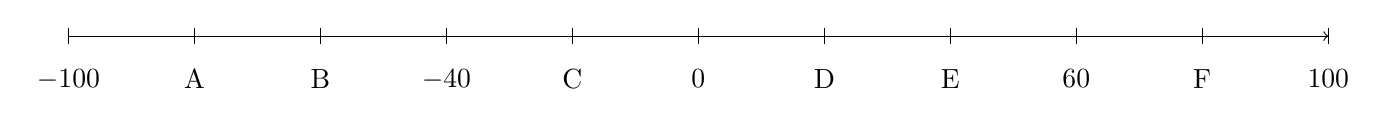
\begin{tikzpicture}[x=0.8cm]  % Set the x unit vector length to 0.8cm
    % Draw the main line
    \draw[->] (-10,0) -- (10,0);
    
    % Draw tick marks and labels
    \foreach \x in {-100, -80, ..., 100} {
        \draw (\x/10,-0.1) -- (\x/10,0.1); % Adjust position for ticks
        % Omit labels at positions -80, -60, -20, 20, 40, and 80 to leave them blank for letters
        \ifnum\x=-80 \else
        \ifnum\x=-60 \else
        \ifnum\x=-20 \else
        \ifnum\x=20 \else
        \ifnum\x=40 \else
        \ifnum\x=80 \else
            \node[below] at (\x/10,-0.3) {$\x$}; % Adjust position for labels
        \fi\fi\fi\fi\fi\fi
    }
    
    % Draw letters 'A', 'B', 'C', 'D', 'E', and 'F' at positions
    \node[below] at (-80/10,-0.3) {A};
    \node[below] at (-60/10,-0.3) {B};
    \node[below] at (-20/10,-0.3) {C};
    \node[below] at (20/10,-0.3) {D};
    \node[below] at (40/10,-0.3) {E};
    \node[below] at (80/10,-0.3) {F};
    
\end{tikzpicture}
\vspace{10pt} \\
\hspace{2.5cm} (ii) Subtract A from F. 
\vspace{10pt}

\item \quad What does 1 represent in this number? Please note that there is a decimal point. 
 \[ 4.715 \]
 
\begin{center}
\begin{tabular}{c@{\hspace{2cm}}c@{\hspace{2cm}}c@{\hspace{2cm}}c}
  Ones & Hundredths & Thousandths & Tenths \\
  \includegraphics[width=1cm]{cross.png} & 
  \includegraphics[width=1cm]{cross.png} & 
  \includegraphics[width=1cm]{cross.png} & 
  \includegraphics[width=1cm]{cross.png} \\
\end{tabular}
\end{center}







\end{enumerate}

\end{document}